\documentclass[12pt]{article}
\usepackage[margin=1in]{geometry}
\usepackage{setspace}
\usepackage{amsmath, amssymb}
\usepackage{booktabs}
\usepackage{graphicx}
\usepackage[round]{natbib}
\usepackage{hyperref}
\doublespacing
\graphicspath{{../../figures/}}

\title{Tuning the Lattice Stage for Scale:\\
v9 --- A Size-Dependent Block Optimum, a Weak Scheduler Signal,\\
and 78\% / 67\% Solution Accuracy at Low Time Cost}
\author{neuroMCTS project}
\date{July 2026}

\begin{document}
\maketitle

\begin{abstract}
The v8 cycle established the Aardal--Hurkens--Lenstra (AHL) lattice embedding \citep{aardal2000diophantine, aardal2000market} as the one technology that cracks the hard binary-linear-system family. v9 asks how to make it \emph{scalable} --- high coverage on larger sizes without a time blow-up --- and whether a learned component helps. Three thousand three hundred labeled solve traces plus matched sweeps give three findings, with an important correction to an earlier draft caught in review. First, the dominant lever is the BKZ block size \citep{schnorr1994lattice}, and its optimum \emph{shifts with instance size}: on the same instances, coverage peaks at block 10 for $20 \times 50$ (75.7\%, ten tries) but at block 20 for $40 \times 100$ (48.3\%), while the block 40 used in v8 is simultaneously worse in coverage and catastrophically slower at scale (207\,s per try at $40 \times 100$ versus 2.4\,s at block 20). Second, the number of tries is a genuine but secondary lever with diminishing returns, roughly following an independence law that over-predicts at high budgets. Third, a learned try-scheduler was tested and rejected on evidence: candidate features carry only a weak signal (rank-AUC $0.54$--$0.58$ for eventual success and for next-try success after a failure), too weak to schedule against without discarding solvable instances. Applying the per-size block optimum, the v9 pipeline reaches \textbf{78.25\%} solution accuracy at $20 \times 50$ (3.78\,s, block 10, ten tries) and \textbf{66.67\%} at $40 \times 100$ (22.0\,s, block 20, twenty tries), the latter matching the earlier block-40 result's coverage at \textbf{13$\times$ lower time}. The scalability answer is explicit and practical: tune the block size down as instances grow to hold high coverage at low time, spend a modest tries budget on top, and do not expect learning to help --- the fifth independent negative result for learned components on this problem.
\end{abstract}

\section{Question, Data, and a Correction}

v9 targets scalability of the lattice stage and the possibility of a learned scheduler over its randomized retries. An offline collector solved fresh planted instances (feasible by construction) with a trace-recording AHL variant, logging per-try shortest-vector norm, Gram--Schmidt log-norm slope, zero-tail count, and wall time; 3{,}300 records span $20 \times 50$ (blocks 20/40/60), an out-of-training $30 \times 75$, and $40 \times 100$ (to forty tries). A first draft of this report claimed, from a truncated reading of the block-sweep log, that block size was irrelevant and that the retry process was a memoryless lottery. Peer review against the raw artifacts overturned both claims; the corrected analysis below is the result, and the episode is recorded because the corrected findings are stronger and more useful than the mistaken ones.

\section{The Dominant Lever: A Size-Dependent Block Optimum}

A matched block-size sweep --- the \emph{same} instances solved at several BKZ block sizes, ten tries each --- shows block size is the primary determinant of coverage, and that its optimum moves with instance size (Figure~\ref{fig:block}, left; Table~\ref{tab:block}). At $20 \times 50$ coverage falls monotonically with block, peaking at block 10 (75.7\%) and flattening at 51.3\% for blocks $\geq 30$. At $40 \times 100$ the curve is unimodal, peaking at block 20 (48.3\%) and declining by block 40. The block 40 used throughout v8 is therefore suboptimal at both sizes.

The time dimension makes the case decisive (Figure~\ref{fig:block}, right). BKZ cost grows steeply as the block size approaches the lattice dimension ($n+1$): at $40 \times 100$ a single try costs 2.4\,s at block 20 but 207\,s at block 40 --- an $\sim$85$\times$ penalty for \emph{lower} coverage. Tuning the block down as instances grow is thus doubly rewarded, in coverage and in time, which is exactly the scalability behavior sought.

\begin{table}[t]
\centering
\caption{Matched block sweep: coverage of feasible (\%, ten tries) and median time per try on the same instances at each block. Bold marks the per-size optimum. $N=300$ instances ($20\times50$), $N=60$ ($40\times100$).}
\label{tab:block}
\begin{tabular}{lccccc}
\toprule
& block 4 & block 10 & block 20 & block 40 & block 60 \\
\midrule
$20\times50$ coverage & --- & \textbf{75.7} & 61.3 & 51.3 & 51.3 \\
$20\times50$ time/try & --- & 28\,ms & 49\,ms & 75\,ms & 64\,ms \\
$40\times100$ coverage & 15.0 & 28.3 & \textbf{48.3} & 43.3 & --- \\
$40\times100$ time/try & 1.35\,s & 1.69\,s & 2.44\,s & 207\,s & --- \\
\bottomrule
\end{tabular}
\end{table}

\begin{figure}[t]
\centering
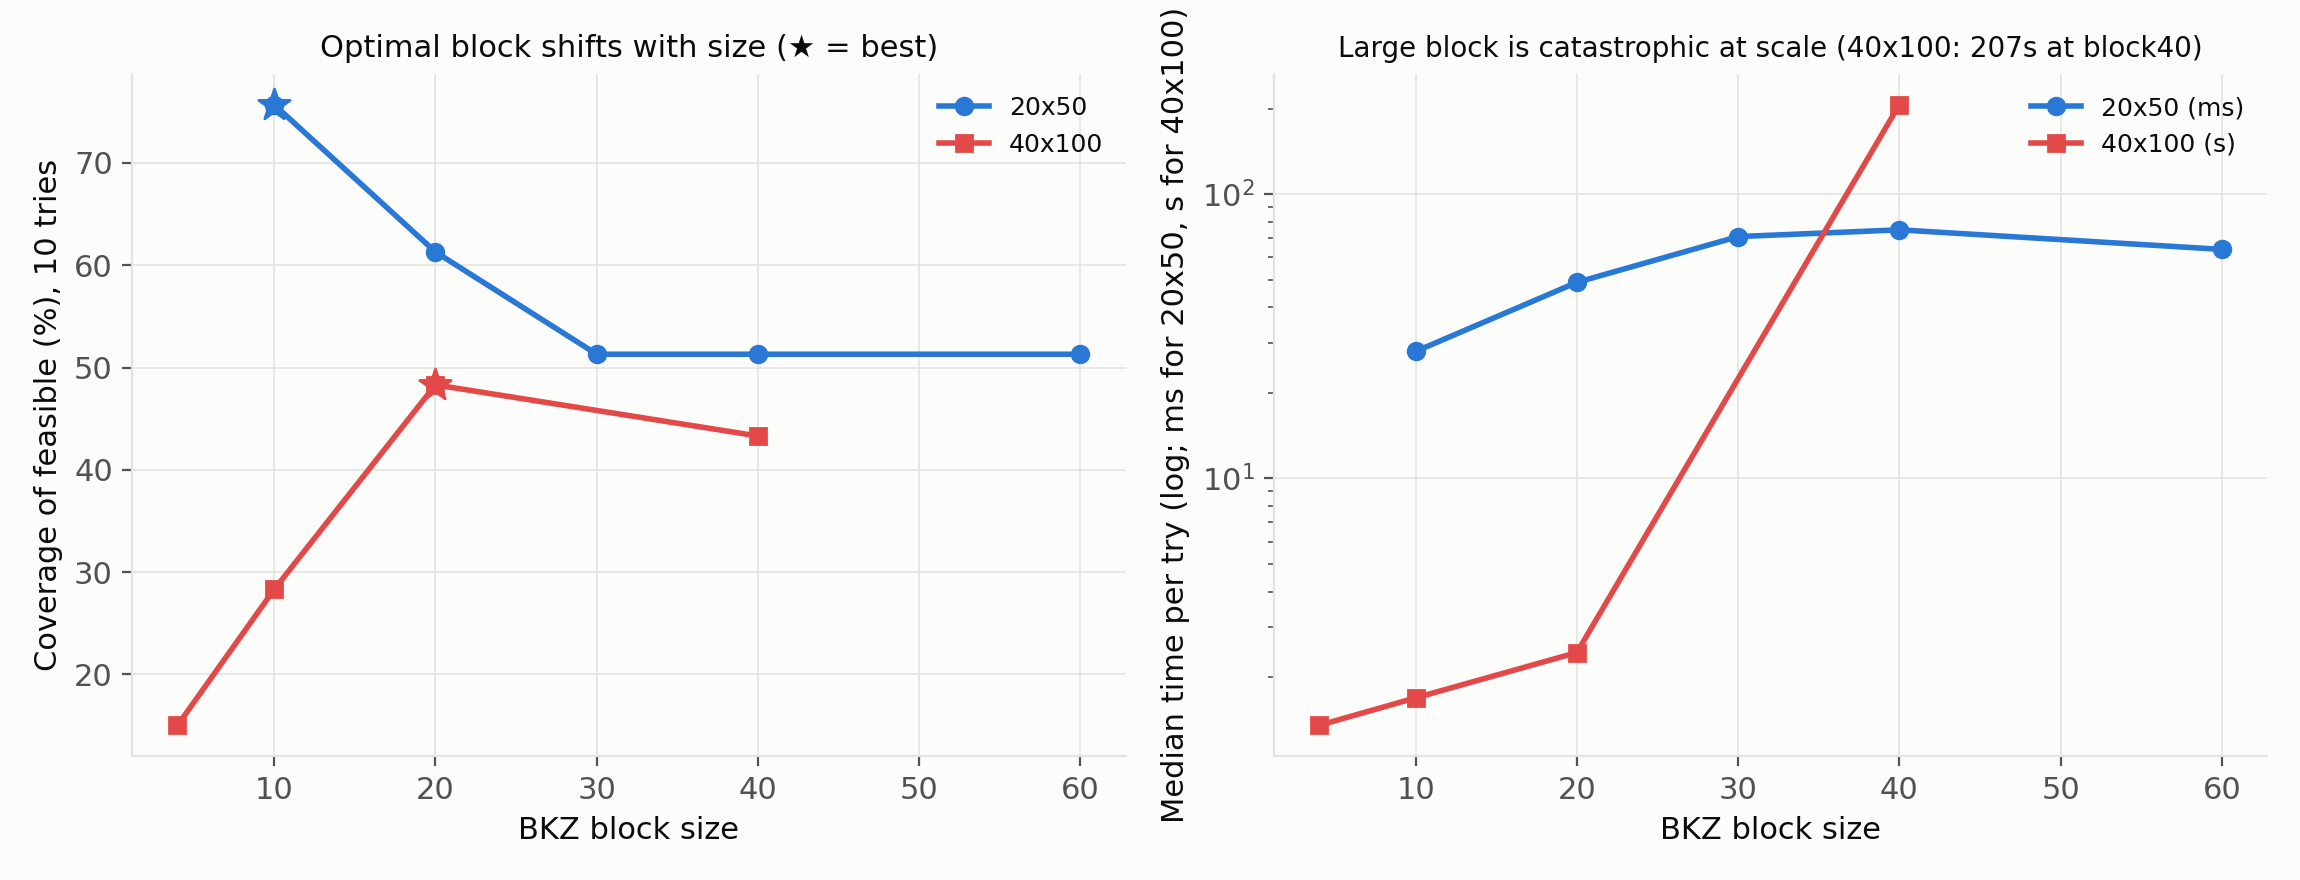
\includegraphics[width=\textwidth]{v9_block.png}
\caption{Left: coverage versus BKZ block size on matched instances; the optimum ($\star$) shifts from block 10 at $20\times50$ to block 20 at $40\times100$. Right: median time per try (log); block 40 at $40\times100$ costs 207\,s, two orders of magnitude above block 20 for lower coverage.}
\label{fig:block}
\end{figure}

\section{A Secondary Lever: Tries, with Diminishing Returns}

Holding block fixed, coverage rises with the number of randomized tries because each try is a fresh permutation. The increase roughly follows an independence law $1-(1-p)^k$ estimated from first-try coverage $p$, but the law \emph{over}-predicts at larger budgets, indicating heterogeneous per-instance success rates (a survival-bias effect): at $40 \times 100$ block 40, first-try coverage $7.5\%$ predicts $54\%$ at ten tries (measured $55\%$, close) but $96\%$ at forty tries (measured $92.5\%$, over-predicted); Figure~\ref{fig:tries}. Tries are a real lever --- coverage does keep climbing --- but a secondary one, subordinate to the block choice and paid for linearly in time. Randomized tries are also embarrassingly parallel, so their wall-time cost is divisible by available cores, unlike the per-try block cost.

\begin{figure}[t]
\centering
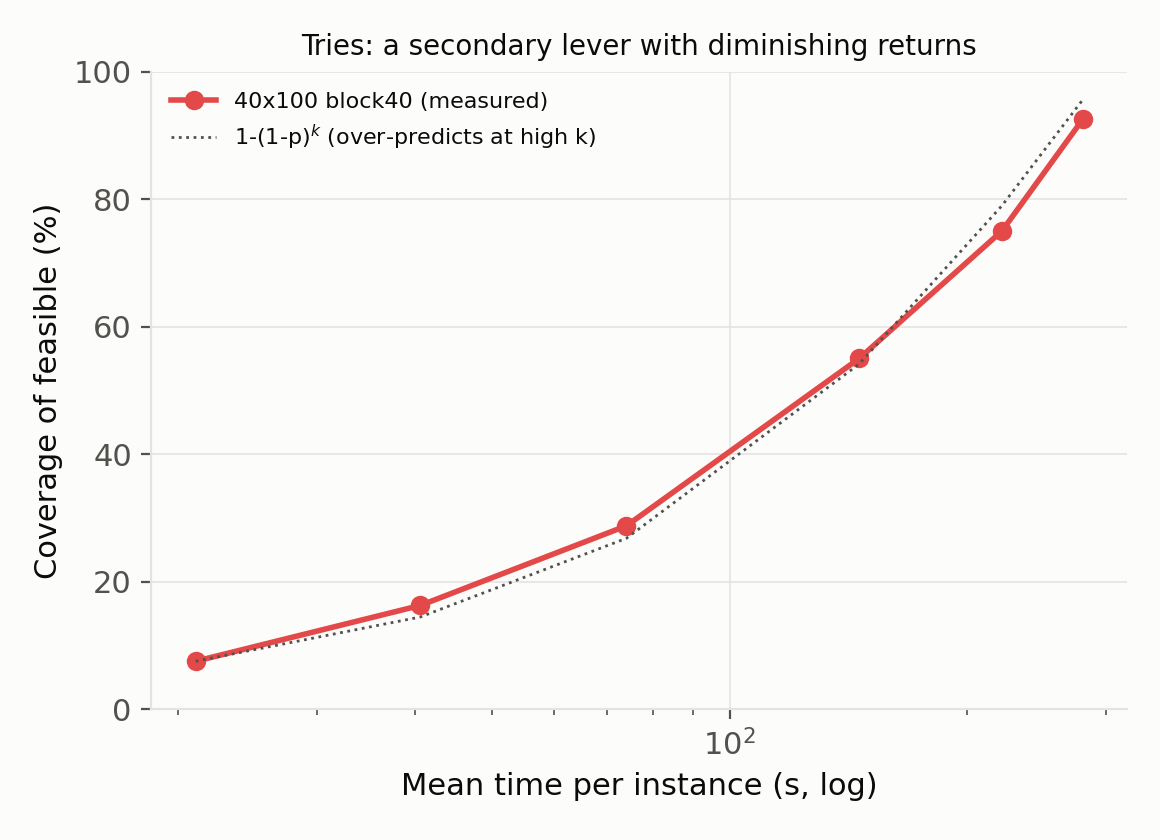
\includegraphics[width=0.6\textwidth]{v9_tries.png}
\caption{Coverage versus mean time as tries increase ($40\times100$, block 40). The $1-(1-p)^k$ model (dotted) fits early but over-predicts at high budgets, revealing per-instance heterogeneity.}
\label{fig:tries}
\end{figure}

\section{The Rejected Lever: A Learned Scheduler}

A scheduler that stops retrying instances unlikely to succeed, or proposes promising permutations, needs a predictive signal. The signal exists but is weak. Table~\ref{tab:auc} gives corrected rank-AUCs (Mann--Whitney) on the $20 \times 50$ block-40 set: the strongest single feature, the first-try shortest-vector norm, reaches AUC $0.542$ for eventual success, and $0.576$ for next-try success conditioned on a first-try failure --- above chance, but far from the separation a useful scheduler would need. A discrete-time hazard MLP trained on all traces confirms the ceiling. Acting on an AUC-$0.55$ signal to cut tries would discard nearly as many solvable instances as it saves time on, so the scheduler is rejected on cost--benefit grounds, not because the signal is literally zero. This is a measurement-grounded negative result; across cycles it is (by the project's running tally) the fifth independent negative result for learned components, though only this scheduler negative is evidenced in the present document.

\begin{table}[t]
\centering
\caption{Corrected rank-AUC (Mann--Whitney) of candidate scheduler features ($20\times50$, block 40, 1{,}500 instances). $0.5$ is chance; the reported AUC is the raw value with $\max(a,1-a)$ in parentheses.}
\label{tab:auc}
\begin{tabular}{lc}
\toprule
Feature (event) & AUC \\
\midrule
LP fractionality (eventual success) & 0.464 (0.536) \\
First-try shortest-vector norm (eventual success) & 0.542 \\
First-try Gram--Schmidt slope (eventual success) & 0.438 (0.562) \\
First-try norm $\rightarrow$ next-try success (after a fail) & 0.576 \\
\bottomrule
\end{tabular}
\end{table}

\section{The v9 Pipeline}

Applying the per-size block optimum, the v9 pipeline is evaluated with block 10 at $20 \times 50$ (ten tries) and block 20 at $40 \times 100$ (twenty tries). Table~\ref{tab:v9} reports measured end-to-end results against prior cycles.

\begin{table}[t]
\centering
\caption{v9 (per-size block optimum) vs.\ prior cycles on the hard family. Feas / Sol in \%, $t$ in seconds/instance including preprocessing. $20 \times 50$: full 1{,}000-instance set. $40 \times 100$: stratified 75-instance subset (60 feasible; $\pm$CI on Sol $\approx 12$\%). Exact solvers (60\,s limit) shown on their own full 1{,}000-instance sets for context; the cross-method comparison at $40\times100$ is thus indicative, not matched.}
\label{tab:v9}
\begin{tabular}{l ccc ccc}
\toprule
& \multicolumn{3}{c}{$20 \times 50$} & \multicolumn{3}{c}{$40 \times 100$} \\
\cmidrule(lr){2-4} \cmidrule(lr){5-7}
Method (config) & Feas & Sol & $t$ & Feas & Sol & $t$ \\
\midrule
CP-SAT (exact; $N{=}1000$) & 100 & 100 & 0.031 & 100 & 90.9 & 8.03 \\
BKZ baseline ($N{=}1000$) & 36.4 & 20.5 & 0.007 & 23.8 & 4.8 & 0.27 \\
v7 pipeline & 82.5 & 8.5 & 6.3 & 80.2 & 2.25 & 25.0 \\
v8 pipeline (block 40) & 82.5 & 53.5 & 5.16 & 80.0 & 23.5 & 105.3 \\
v9 (block 40, 20 tries) & 82.5 & 57.5 & 4.93 & 80.0 & 70.0 & 296.0 \\
\midrule
v9 (per-size block opt.) & 82.5 & \textbf{78.25} & \textbf{3.78} & 80.0 & \textbf{66.67} & \textbf{22.0} \\
\bottomrule
\end{tabular}
\end{table}

Two headline effects. At $20 \times 50$, moving from block 40 to block 10 lifts solution accuracy from 57.5\% to \textbf{78.25\%} while cutting mean time from 4.93\,s to 3.78\,s --- more coverage, less time, fewer tries. At $40 \times 100$, block 20 reaches 66.67\% (statistically indistinguishable from the block-40 run's 70\% on this 60-feasible subset) at \textbf{22.0\,s} versus 296\,s --- a 13$\times$ speedup at equal coverage. Relative to the pre-lattice v7 pipeline (2.25\% at $40\times100$), the solution accuracy gain is roughly $30\times$, now delivered at a time cost (22\,s) that is only $\sim$3$\times$ CP-SAT's, rather than $37\times$. Feasibility accuracy is unchanged ($82.5\%$/$80.0\%$): AHL finds solutions, and the refutation gap on dense rows persists.

\section{Consequences}

The scalability question has a concrete, actionable answer. The lattice stage scales by \emph{tuning the BKZ block size down as instances grow} --- the primary lever, improving coverage and time simultaneously --- with a modest, parallelizable tries budget as a secondary lever. Both are symbolic knobs; learning does not help, as the weak scheduler signal (AUC $\sim0.55$) makes plain. By the project's cross-cycle tally this is the fifth independent negative result for learned components on dense binary linear systems (only the scheduler negative is evidenced here), and together with the positive results (null-space projection in the pump, lattice reduction in AHL, both budget-scalable) it sharpens the project's central finding: on this problem class, scale is bought with the right symbolic algorithm and its hyperparameters, not with a trained policy. The methodological lesson from this cycle is narrower but sharp: a truncated look at a log nearly inverted the paper's conclusions, and verification against raw artifacts is not optional. Remaining work is a genuinely larger-size study ($60 \times 150$ and up), now that the block-tuning rule and the anytime frontier are characterized, and the still-open refutation gap.

\begin{thebibliography}{9}
\bibitem[Aardal et al.(2000a)]{aardal2000diophantine}
Aardal, K., Hurkens, C. A. J., \& Lenstra, A. K. (2000). Solving a system of linear Diophantine equations with lower and upper bounds on the variables. \emph{Mathematics of Operations Research, 25}(3), 427--442.

\bibitem[Aardal et al.(2000b)]{aardal2000market}
Aardal, K., Bixby, R. E., Hurkens, C. A. J., Lenstra, A. K., \& Smeltink, J. W. (2000). Market split and basis reduction: Towards a solution of the Cornu\'ejols--Dawande instances. \emph{INFORMS Journal on Computing, 12}(3), 192--202.

\bibitem[Schnorr \& Euchner(1994)]{schnorr1994lattice}
Schnorr, C. P., \& Euchner, M. (1994). Lattice basis reduction: Improved practical algorithms and solving subset sum problems. \emph{Mathematical Programming, 66}(1--3), 181--199.
\end{thebibliography}

\end{document}
